\chapter{Θεωρητικό Υπόβαθρο}

\section{\en{Unikernels - Rumprun}}

\subsection{Ορισμός}

Ο όρος \en{unikernel} αναφέρεται σε μικρές, εξειδικευμένες εικονικές μηχανές,
χωρίς διαχωρισμό \en{user space} και \en{kernel space}, τα οποία κατασκευάζονται
χρησιμοποιώντας κάποιο \en{library operating system}\cite{unikernelsDef}.
\newline

Αυτές εικονικές μηχανές είναι μικρές σε μέγεθος, καθώς συνήθως έχουν
αφαιρεθεί πολλαπλά στρώματα-μέρη λογισμικού που υπάρχουν σε ένα παραδοσιακό
λειτουργικό σύστημα. Εξειδικευμένες, επειδή εστιάζουν στην εκτέλεση μιας
και μόνο λειτουργίας, και δεν προσφέρουν δυνατότητες παράλληλης εκτέλεσης
πολλαπλών εφαρμογών όπως τα παραδοσιακά λειτουργικά συστήματα. Το πιο
σημαντικό, όμως, χαρακτηριστικό είναι η ανάπτυξη τους χρησιμοποιώντας
κάποιο \en{library operating system}, το οποίο και αξίζει να αναλυθεί στην συνέχεια.






%ΛΙΒΡΑΡΥ ΟΠΕΡΤΙΝΓ ΣΥΣΤΕΜΣ
\subsection{\en{Library Operating System}}

Τα \en{library operating systems} αποτελούν μια μορφή αρχιτεκτονικής
όπου οι διάφορες υπηρεσίες που χρειάζεται ένα \en{high level }
\en{application}, για παράδειγμα αν επιθυμεί να ανταλλάσει πακέτα
με χρήση κάποιου \en{network protocol}, προσφέρονται ως συναρτήσεις
βιβλιοθήκης από το περιβάλλον στο οποίο αναπτύσσεται, οι οποίες
ενσωματώνονται τελικά σε ένα μοναδικό επίπεδο λογισμικού. Για
να μπορεί να επιτευχθεί αυτό, τα \en{library operating systems}
από σχεδιασμού τους προσφέρουν δύο πράγματα. Πρώτον τις βιβλιοθήκες
οι οποίες προσφέρουν πρόσβαση στο υλικό και στους πόρους,
ουσιαστικά τον μηχανισμό. Δεύτερον, τις κατάλληλες πολιτικές με
τις οποίες επιτυγχάνεται ορθός έλεγχος της πρόσβασης, και απομόνωση
στο υψηλό επίπεδο της εφαρμογής. Ο έλεγχος, συνεπώς, και η προστασία
του υλικού δεν εξασφαλίζεται πλέον μεταξύ του χώρου της
εφαρμογής και του χώρου του πυρήνα του λειτουργικού, αλλά ακόμα
χαμηλότερα, στο επίπεδο του υφιστάμενου υλικού\cite{riseOfVirtLibOS}.
\newline

Οι πρώτες υλοποιήσεις τέτοιων συστημάτων-αρχιτεκτονικών,
εμφανίστηκαν στα τέλη της δεκαετίας του 1990, όπως το \en{Exokernel}
και το \en{Nemesis}\cite{riseOfVirtLibOS}. Ένα εμφανές πλεονέκτημα αυτών των
λιγότερων σύνθετων αρχιτεκτονικών, είναι η ταχύτερη πρόσβαση
στους πόρους, καθώς δεν χρειάζεται η εναλλαγή μεταξύ
\en{privilege mode} και μη. Κυρίως, όμως, η απλούστευση σε επίπεδου
στοίβας λογισμικού προσφέρει προβλέψιμη συμπεριφορά όλου του
συστήματος, και οδηγεί σε σταθερότερες και ασφαλέστερες εφαρμογές.
\newline

Κληρονομώντας, συνεπώς, αυτήν την φιλοσοφία τα \en{unikernels} στηρίζονται
επάνω σε αυτή την απλούστευση της στοίβας του λογισμικού. Το
ερώτημα, λοιπόν, που οδήγησε στην δημιουργία των \en{unikernel},
είναι το εξής: «τι θα γινόταν αν ολόκληρη η στοίβα του λογισμικού,
από το ανώτερο επίπεδο, μέχρι και τον κώδικα \en{assembly},
μεταγλωτίζονταν ως ένα σώμα σε ένα ασφαλές, υψηλού επιπέδου γλωσσας \en{framework};»







%ΧΑΡΑΚΤΗΡΙΣΤΙΚΑ
\subsection{Χαρακτηριστικά}

Για να γίνει καλύτερα κατανοητή η διαφορά και το πλεονέκτημα ενός
\en{unikernel} σε σχέση με ένα συμβατικό λειτουργικό σύστημα, θα
συγκριθεί στην συνέχεια η στοίβα λογισμικού σε δύο διαφορετικές περιπτώσεις.
\newline

Σε ένα παραδοσιακό λειτουργικό σύστημα όπως στο \en{linux}, ο
προγραμματιστής αναπτύσσει τον κώδικα της εφαρμογής του στο
υψηλότερο επίπεδο. Ο κώδικας αυτός εξαρτάται εν πολλοίς από
διάφορες βιβλιοθήκες που προσφέρει το σύστημα. Αυτές οι
βιβλιοθήκες ενώνονται δυναμικά ή στατικά με τον κώδικα του χρήστη και παράγεται το
εκτελίσμο της εφαρμογής. Τώρα, κατά την εκτέλεση η εφαρμογή
επικοινωνεί με τον πυρήνα του λειτουργικού συστήματος ώστε αυτός
να εκτελέσει με την σειρά του προνομιούχες εντολές-διαδικασίες οι οποίες
σχετίζονται με λειτουργίες οι οποίες σε ένα \en{multi-process}
περιβάλλον χρήζουν ασφαλείας και προσοχής. Χαρακτηριστικό παράδειγμα είναι
ή πρόσβαση στο υλικό, όπως π.χ. μια ανάγνωση από αρχεία του δίσκου. Ο μηχανισμός
που διεκπεραιώνει αυτήν την επικοινωνίας είναι οι κλήσεις συστήματος
(\en{system calls}), σύμφωνα με τις οποίες η εκτελούμενη
διεργασίας υποχρεούται να αιτηθεί από τον
πυρήνα (\en{kernel}) του λειτουργικού να αναλάβει την ενέργεια εκ μέρους
της. Υποχρεωτικά εμφανίζεται αυτός ο διαχωρισμός
μεταξύ του χώρου χρήστη και του χώρου πυρήνα, και για κάθε
προνομιούχα δραστηριότητα πρέπει να γίνεται εναλλαγή (\en{context switch}) μεταξύ
αυτών των δύο. Ακόμα πιο κάτω, υπάρχει ο κώδικας που τρέχει
στον χώρο πυρήνα, από το σύστημα αρχείων, τις εικονικές
συσκευές,τους \en{drivers} που επικοινωνούν με το το πραγματικό υλικό
έως και την διαχείριση μνήμης και την χρονοδρομολόγηση των διεργασιών.
\newline

Από την άλλη, σε ένα \en{unikernel} περιβάλλον εκτελείται μονάχα
μία εφαρμογή χωρίς την πιθανή συνεκτέλεση τρίτων εφαρμογών. Για αυτό τον
λόγο, απουσιάζει ο διαχωρισμός ανάμεσα σε \en{user space} και
\en{kernel space}, καθώς δεν υπάρχει ανάγκη προστασίας και ασφάλειας
μεταξύ διεργασιών. Αυτό οδηγεί, σε ένα μοναδικό χώρο όπου ο
κώδικας από το πιο υψηλό επίπεδο μέχρι και το πιο χαμηλό
εκτελείται σε μοναδικό \en{context} και χώρο διευθύνσεων μνήμης.
Ταυτόχρονα, κατά την μεταγλώττιση της εφαρμογής, το \en{toolchain}, δηλαδή
τα εργαλεία δημιουργίας του \en{unikernel}, του εκάστοτε
\en{unikernel framework}, αφαιρεί όλα τα περιττά συστατικά του
συστήματος, ώστε να απομένουν τα απολύτως απαραίτητα που
χρειάζονται για τον συγκεκριμένο σκοπό. Απουσιάζει, επίσης, το
σύστημα που διαχειρίζεται την παράλληλη εκτέλεση των
διεργασιών και συνήθως η εικονική μνήμη\cite{libOSCloud}.
\newline

\begin{figure}[h]
  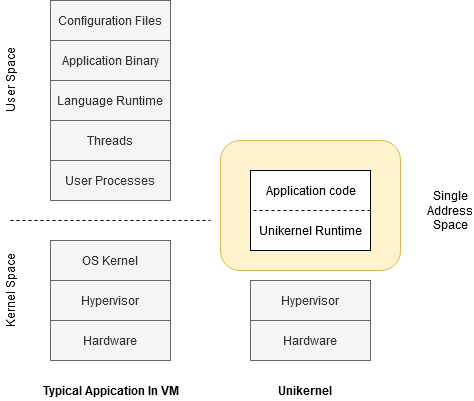
\includegraphics[width=\textwidth]{pictures/UnikernelDesign.png}
  \caption{Συμβατική εικονική μηχανή - \en{Unikernel}}
  \label{fig:genUnikernel}
\end{figure}

Δημιουργείται, συνεπώς, μια ταχύτατη, μικρή και εστιασμένη
εικονική μηχανή, η οποία μπορεί να εκτελεστεί αυτόνομα
επάνω σε ένα \en{hypervisor} ή στο ίδιο το υλικό, δίχως την
ανάγκη ενός υφιστάμενου λειτουργικού συστήματος. Η εκκίνηση
(\en{boot}) είναι ταχύτατη, τάξης μεγέθους ανώτερη από ένα
συμβατικό λειτουργικό στο οποίο εκτελείται αντίστοιχη
εφαρμογή. Ταυτόχρονα, η ασφάλεια είναι αυξημένη καθώς η
εφαρμογή τρέχει στο δικό της περιβάλλον, αποκομμένη από
την συνεκτέλεση άλλων στο ίδιο χώρο χρήστη, όπως ισχύει στα συμβατικά
λειτουργικά συστήματα. Τέλος, οι
ανάγκες σε πόρους ελαχιστοποιούνται, καθώς μπορεί να ανατεθούν
ακριβώς όσους χρειάζεται η συγκεκριμένη εφαρμογή,
ενώ σε ένα συμβατικό λειτουργικό θα έπρεπε να μεριμνήσει ο σχεδιαστής ώστε
να υπάρχουν διαθέσιμοι πόροι για όλες τις εφαρμογές που μπορεί
να εκτελεστούν παράλληλα, ακόμα και αν δεν εκτελούνται πράγματι.







%FRAMEWORKS
\subsection{\en{Frameworks}}

Ακολουθεί μια χρήσιμη αναφορά σε διάφορα \en{unikernel framework}
που υπάρχουν την στιγμή που γράφονται αυτές οι γραμμές,
καθώς και μια ανάλυση των χαρακτηριστικών του καθενός.

\subsubsection{\en{MirageOs}}

Το \en{MirageOs} αποτελεί ένα από τα παλαιότερα και πιο διαδεδομένα
\en{frameworks}. Το \en{MirageOs} δημιουργήθηκε στο εργαστήριο
υπολογιστών του πανεπιστημίου του \en{Cambridge}. Ο σκοπός των δημιουργών ήταν
να λύσουν το
πρόβλημα που προκύπτει κατά την εικονικοποίηση συστημάτων, πως
προστίθεται ένα επιπλέον στρώμα λογισμικού, οδηγώντας σε μη
βέλτιστη συμπεριφορά των εικονικών μηχανων\cite{riseOfVirtLibOS}. Μάλιστα στο
ίδιο εργαστήριο είχε αναπτυχθεί το 2003 ο \en{hypervisor Xen}\cite{xenArtofVirt}.
Ο σκοπός του \en{project}, είναι να ανακατασκευαστούν οι εικονικές
μηχανές, από το επίπεδο της εφαρμογής μέχρι και το επίπεδο
του πυρήνα ώστε να είναι καλύτερα αλληλοσυνδεδεμένα στην βάση
ενός \en{library operating system}.
\newline

Για την δημιουργία του \en{unikernel} με βάση το \en{MirageOS}
χρησιμοποιείτε η γλώσσα
\en{OCaml}, μια γλώσσα αρκετά υψηλού επιπέδου. Η επιλογή της
συγκεκριμένης γλώσσας έχει γίνει διότι αυτή επιτρέπει την
ανάπτυξη \en{type safe} εφαρμογών με μέλημα την προστασία της
μνήμης από \en{memory leaks}. Τέτοια σφάλματα σχετίζονται με
την μη ορθή χρήση των διαφόρων τύπων δεδομένων από μια γλώσσα.
Η \en{OCaml} για να το πετύχει αυτό διαθέτει στατικό έλεγχο των
τύπων (\en{static type check}), οπότε οι τυχόν ασυμφωνίες εντοπίζονται
κατά το \en{compile} και όχι κατά την εκτέλεση, καθώς και ένα
διακριτικό συλλέκτη σκουπιδιών (\en{garbage collector}), ο οποίος
ανακυκλώνει την αποδεσμευμένη μνήμη.
\newline

Για να αξιοποιηθούν καλύτερα τα νέα χαρακτηριστικά του \en{mirageOs},
αναπτύχθηκαν από την αρχή σημαντικά συστατικά ενός παραδοσιακού
λειτουργικού συστήματος, όπως το \en{network} και \en{storage stack}.
Έτσι, γράφτηκαν βιβλιοθήκες για \en{TCP/IP, ΗΤΤP, DNS} κ.α. στην
\en{Ocaml}. Το αποτέλεσμα είναι ένα ασφαλές και αρθρωτό \en{framework},
ιδανικό να υποστηρίξει \en{web υπηρεσίες}. Υπάρχουν διάφορα
παραδείγματα \en{self-hosted} διαδικτυακών ιστοσελίδων που εκτελούνται
ως \en{MirageOs} εφαρμογές επάνω σε κάποιον \en{hypervisor}, όπως το \en{Xen}\cite{overMirage}.
\newline

Ένα μειονέκτημα είναι πως η εκτελούμενη εφαρμογή πρέπει να
είναι γραμμένη σε \en{OCaml} για να μπορεί να εκτελεστεί με το
\en{MirageOs}. Αυτό συνήθως δεν ισχύει για τα περισσότερα
προγράμματα, με αποτέλεσμα να απαιτείται ανάπτυξη της εφαρμογής
από την αρχή. Τέλος, οι υποστηριζόμενες πλατφόρμες είναι το
\en{Xen}, και το \en{KVM} αν χρησιμοποιηθεί το \en{solo5 framework}, που
θα αναλυθεί στην συνέχεια.

\subsubsection{\en{IncludeOS}}

Το \en{IncludeOS} είναι ένα μινιμαλιστικό, ανοιχτού κώδικα, \en{unikernel}
\en{framework}, το οποίο στοχεύει σε εφαρμογές και υπηρεσίες
γραμμένες σε γλώσσα \en{C++}, και που στοχεύουν στο \en{cloud}. Πρόκειται
για ένα από τα νεότερα \en{unikernel frameworks}, και στοχεύει στην
ανάπτυξη τέτοιων εικονικών μηχανών με την ευκολία που έχει η
συμπερίληψη μια βιβλιοθήκης κατά την ανάπτυξη των εφαρμογών.
Γράφοντας απλά \en{\#include<os>}, κυριολεκτικά κατά το \en{linking} της
εφαρμογής μας θα συμπεριληφθεί ένα μικροσκοπικό λειτουργικό
σύστημα και θα παραχθεί μια πλήρης εικόνα εικονικής μηχανής\cite{includeOS}.
\newline

Σε αντίθεση με αρκετά άλλα \en{frameworks}, το\en{ IncludeOs} δεν έχει
κληρονομήσει από κάποιο άλλη πλατφόρμα αυτούσιες τις
βιβλιοθήκες ή και τα συστατικά στοιχεία που χρειάζονται οι εφαρμογές.
Αντίθετα όλα αυτά έχουν γραφτεί από την
αρχή σε \en{C++}, με έμφαση στα \en{unikernel} χαρακτηριστικά του.
Με αυτόν τον τρόπο έχει επιτευχθεί αποδοτική διαχείριση
των πόρων και των απαιτήσεων σε μνήμη, αποδοτική διαδικασία
\en{deployment}, και ανεξαρτησία από την πλατφόρμα εικονικοποίησης.
Αυτή την στιγμή τα \en{unikernel} που παράγονται από το
\en{IncludeOs} μπορούν να εκτελεστούν επάνω στους περισσότερους
δημοφιλείς επόπτες, καθώς και στο \en{openStack}\cite{Orestis}.
\newline

Το \en{IncludeOs} χαρακτηρίζεται από χαμηλό αποτύπωμα μνήμης,
υποστήριξη για \en{C++11/17}, τις κλασσικές βιβλιοθήκη \en{C++} κ.α..
Επίσης, υπάρχει υποστήριξη και για την βιβλιοθήκη της \en{C}
γλώσσας, δίνοντας μια συμβατότητα με κάποιες \en{POSIX} εφαρμογές\cite{includeOS}.
Τέλος, είναι αρκετά ενδιαφέρον το γεγονός πως υλοποιήθηκε από την αρχή
μια αρθρωτή στοίβα δικτύου εστιασμένη στο \en{project}, που
επιτρέπει ταχύτερη ανταλλαγή πακέτων και υψηλότερη απόδοση.
\newline

Μια εφαρμογή σε \en{IncludeOs}, δεν εκκινεί όπως μια παραδοσιακή
εφαρμογή για συμβατικό λειτουργικό με μια \en{main()}, αλλά με
την εντολή \en{Service::start}. Αυτό πρόκειται την υπηρεσία
(\en{service)} που οφείλει να υλοποιεί ο προγραμματιστής αν θέλει
να εκκινήσει η εφαρμογή του. Οι εφαρμογές πρέπει να γράφονται
υποχρεωτικά σε γλώσσα \en{C++}. Όπως και στα περισσότερα
\en{unikernel framework}, δεν υπάρχει υποστήριξη για εικονική
μνήμη ούτε ο διαχωρισμός μεταξύ \en{user space} και \en{kernel space}.
Τέλος, εφόσον απουσιάζουν τα νήματα και εκτελείται
κώδικας μόνο μιας διεργασίας, πολυνηματικές εφαρμογές ή εφαρμογές
που στηρίζονται στην παράλληλη εκτέλεση πολλών εργασιών
πρέπει να ξαναγραφούν ώστε να ταιριάζουν με τα
χαρακτηριστικά του \en{framework}\cite{Charalampos}.

\subsubsection{\en{OSv}}

Το \en{OSv} αποτελεί ένα σύγχρονο λειτουργικό σύστημα το οποίο
εστιάζει στην εκτέλεση των εφαρμογών στο \en{cloud}.
Δημιουργήθηκε το 2013 από την \en{Cloudious Systems} με σκοπό
να τρέχει επάνω σε μια πληθώρα από \en{hypervisors}, και να
υποστηρίζει τις περισσοτερες από τις δημοφιλείς γλώσσες,
\en{C, C++, Java, Ruby, NodeJS} κλπ. Πρόκειται, συνεπώς, για
ένα \en{unikernel framework} ικανό να εκτελέσει  \en{single-process linux}
εφαρμογές\cite{Orestis}.
\newline

Σε σχέση με τα υπόλοιπα \en{unikernel frameworks}, το \en{OSv}
χαρακτηρίζεται ως ένα λειτουργικού γενικού σκοπού, που
μπορεί να μετατρέψει σχεδόν κάθε εφαρμογή σε \en{unikernel}.
Ταυτόχρονα, υποστηρίζει τους περισσότερους γνωστούς
επόπτες, όπως \en{Xen, KVM, QEMU, VMware, GCE}. Αυτή η ιδιότητα το
υποχρεώνει να είναι ένα από το πιο σύνθετα, και συνεπώς
μεγάλα σε μέγεθος, \en{unikernel}, όπου η παραγόμενη εικονική
μηχανή είναι τάξης μερικών δεκάδων \en{megabytes}. Εν συγκρίσει, τα περισσότερα
\en{unikernels} εμφανίζουν συνηθισμένο μέγεθος μερικών \en{kilobytes}\cite{Orestis}.
\newline

Όπως και στα περισσότερα \en{unikernel} περιβάλλοντα, υπάρχει
μόνο μια εκτελούμενη διεργασία ανά πάσα στιγμή και
απουσιάζει ο διαχωρισμός \en{user space} και \en{kernel space},
οπότε όλος ο κώδικας τρέχει σε ένα μοναδικό χώρο μνήμης.
Αυτό προφανώς οδηγεί στην μείωση της καθυστέρησης της
εκτέλεσης που σχετίζεται με την αλλαγή του \en{context}.
\newline

Ένα αξιοσημείωτο χαρακτηριστικό του είναι η χρήση
χρονοδρομολογητή (\en{scheduler}) για τον συγχρονισμό
των εικονικών επεξεργαστών (\en{virtual CPUs}), χωρίς την
χρήση \en{spinlocks}. Tα \en{spinlocks} χρησιμοποιούνται όταν
τα νήματα που πρέπει να συγχρονιστούν ως προς την
πρόσβαση σε ένα κοινόχρηστο πόρο, όπως π.χ. μια ευαίσθητη
περιοχή μνήμης, δεν μπορούν να κοιμηθούν. Στα
εικονικοποιημένα περιβάλλοντα είναι όμως πιθανόν
μια εικονική \en{CPU} να πάψει προσωρινά να εκτελεί
εντολές, με αποτέλεσμα να υποχρεώνει τις υπόλοιπες
να αναμένουν άεργες σπαταλώντας πόρους. Επιλέχθηκε,
συνεπώς, όλα τα νήματα στο \en{OSv}, εκτός από τον ίδιο τον \en{scheduler},
να είναι σε θέση να κοιμηθούν, και άρα να μην απαιτούνται
\en{spinlocks}\cite{OSV-optimizing}. Επίσης, δεδομένου πως η εκτέλεση διαδικτυακών
εφαρμογών στο \en{cloud} θα είναι ο κύριος στόχος τέτοιων \en{frameworks},
οι συσκευές δικτύου σχεδιάστηκαν από την αρχή. Με την
τεχνική που ονομάζεται κανάλια δικτύου (\en{network channels}),
τα πακέτα που έρχονται με διακοπές από το δίκτυο
επεξεργάζονται και ταξινομούνται σε ξεχωριστά νήματα,
μέσα στο ίδιο \en{context} με την εκτελούμενη εφαρμογή
επιτυγχάνοντας αυξημένη επίδοση ταχύτητα, απλοποιώντας
τον ανταγωνισμό για τους μηχανισμούς από τα διάφορα περιβάλλοντα επικοινωνίας
που χρησιμοποιούν το δίκτυο. Τέλος, πολύ ενδιαφέρον είναι
πως, σε αντίθεση με τα αρκετά άλλα \en{unikernel frameworks},
στο \en{OSv} υπάρχει υποστήριξη για εικονική μνήμη. Έτσι
εφαρμογές που στηρίζονται σε αυτή, π.χ. με χρήση της
\en{mmap()}, μπορούν να μετατραπούν πιο εύκολα σε \en{unikernel}\cite{OSV-optimizing}.

\subsubsection{\en{Solo5}}

Το \en{Solo5} δεν πρόκειται για ένα πλήρες \en{unikernel framework}, όπως
τα υπόλοιπα που αναφέρονται στην παρούσα εργασία, αλλά ένα ενδιάμεσο
στρώμα επάνω στο οποίο μπορεί να αναπτυχθεί ένα \en{unikernel}.
Ξεκίνησε από τον \en{Dan Williams} της \en{IBM Research}, με σκοπο να
επιτρέψει στο \en{MirageOs} να εκτελείται επάνω στον επόπτη \en{linux-KVM}.
Πλέον έχει εξελιχθεί σε ένα \en{sandbox} περιβάλλον εκτέλεσης και
απομόνωσης επάνω στο οποίο μπορεί να εκτελεστεί ένα μεγάλος
αριθμός από \en{Unikernel} ή γενικότερα από \en{library operating systems}.
Μπορούμε να το φανταστούμε ως ένα στρώμα λογισμικού, το οποίο
κάθεται ανάμεσα στον επόπτη και στο \en{Unikernel}\cite{solo5}.
\newline

Όπως έχει αναφερθεί, βασικό συστατικό της φιλοσοφία των \en{Unikernel},
και γενικώς των \en{library operating systems}, είναι η αφαίρεση
των περιττών συστατικών που υπάρχουν σε ένα συμβατικό
λειτουργικό. Το \en{Solo5} πηγαίνει αυτή την ιδέα ένα βήμα παραπέρα,
θεωρόντας τώρα όλο το \en{unikernel} ως μια διεργασία της οποίας
η διεπαφή με το \en{hypervisor} ή και γενικά με όλο το λειτουργικό
σύστημα επανασχεδιάζεται. Αρχικά, είναι επιθυμητό η διεπαφή να είναι
\en{lightweight} και όσο πιο δυνατόν \en{legacy-free}. Για παράδειγμα
το \en{QEMU}, ένα από τα πιο δημοφιλή \en{hypervisors}, εκθέτει
στο \en{unikernel} μια πληθώρα από εικονικές συσκευές, άχρηστες
για το \en{unikernel}, ακριβώς επειδή το \en{QEMU} είναι σχεδιασμένο
να υποστηρίζει πλήρη λειτουργικά συστήματα και όχι αποκλειστικά
\en{unikernel}\cite{solo5Monitor}. Το \en{Solo5} περιορίζει την διεπαφή μόνο στα
συστατικά που χρειάζεται το \en{unikernel}. Το κέρδος είναι πως με την
αυξημένη αφαίρεση μπορούμε να πετύχουμε μεγαλύτερη φορητότητα
(\en{portability}) των \en{unikernel} ανάμεσα σε διάφορες πλατφόρμες\cite{Orestis}.
Είναι εμφανής η αναλογία των σχέσεων μεταξύ διεργασίας-λειτουργικού
και \en{unikernel-hypervisor}.
\newline

Επιπροσθέτως, το \en{Solo5} εισάγει την έννοια του προγράμματος
φύλακα (\en{tender}), το οποίο ονομάζει \en{hvt (harware virtualized tender)}.
Ο φύλακας είναι ένα εξειδικευμένα στρώμα διεπαφής για \en{unikernels}.
Ο ρόλος του μοιάζει με αυτόν που έχει παραδοσιακά το \en{QEMU}, όμως
όπως αναφέρθηκε, το \en{QEMU} είναι γενικού σκοπού, ενώ ο \en{hvt}
στοχεύει σε ένα συγκεκριμένο \en{unikernel}. Το \en{interface}, λοιπόν,
που ‘βλέπει’ το \en{unikernel} είναι αυτό ακριβώς που έχει το ίδιο
ανάγκη, και τίποτα παραπάνω, μειώνοντας έτσι την επιφάνεια
επίθεσης και το ενδεχόμενο κάτι να δυσλειτουργήσει.
\newline

Το κέρδος αυτής της μείωσης της επιφάνειας του \en{interface}, είναι
πολύ σημαντικό. Η μη ανάγκη για αρχικοποίηση των περιττών
στοιχείων επιτρέπει στα \en{unikernel} να εκκινούν (\en{boot}) αισθητά
πιο γρήγορα από άλλα. Η ασφάλεια βρίσκεται σε υψηλότερα επίπεδα,
καθώς δεν υπάρχουν περιττά \en{components}, με τα οποία θα μπορούσε
κάποιος να επηρεάσει το \en{unikernel}. Τέλος, το σύνολο \en{unikernel-monitor},
μειώνεται δραματικά σε μέγεθος, καθώς δεν χρειάζεται η παρουσία
ενός \en{general-purposed} και ‘βαριού’ \en{monitor} όπως το \en{QEMU}, αλλά ένα
\en{lightweight} και γρήγορου\cite{solo5Monitor}\cite{Orestis}.
\newline

\begin{figure}[h]
  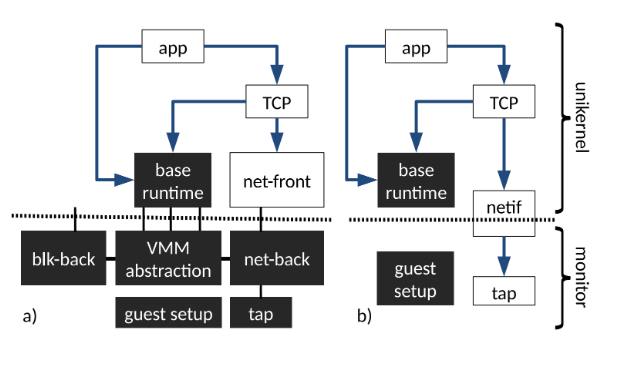
\includegraphics[width=\textwidth]{pictures/unikern-unikernel+monitor(solo5).PNG}
  \caption{\en{a. Monitor} γενικού σκοπού \en{b. Monitor} ειδικού σκοπού}
  \label{fig:solo5}
\end{figure}


Το \en{Solo5} χρησιμοποιείται κυρίως από το \en{MirageOS}, που ήταν και ο
αρχικός στόχος του, και από το \en{IncludeOS}. Επίσης υποστηριζόμενες
πλατφόρμες-\en{hypervisors} είναι \en{linux-KVM, FreeBSD-VMM} ως \en{hvt},
και γενικά οποιοσδήποτε \en{hypervisor} σε \en{x}86 αρχιτεκτονική αρκεί
να υποστηρίζει με την σειρά του \en{virtio} συσκευές, όπως \en{QEMU/KVM}\cite{Orestis}.
Σημειώνεται επίσης, πως το \en{solo5 } ούτε στοχεύει ούτε υποστηρίζει την
απευθείας εκτέλεση στο υλικό (\en{bare-metal}).

\subsubsection{\en{Rumprun}}

Το \en{Rumprun} αποτελεί ένα \en{unikernel framework}, που έχει στηριχθεί
επάνω στα \en{rump kernels} και στοχεύει στην εκτέλεση οποιαδήποτε
\en{single-process POSIX} εφαρμογής. Αυτή είναι και η ιδέα που ώθησε
την δημιουργία του, δηλαδή να μπορεί να μετατραπεί οποιαδήποτε
\en{POSIX} εφαρμογή σε \en{unikernel}, με όσο τον δυνατόν ελάχιστες αλλαγές
στον κώδικά της\cite{Orestis}\cite{RumprunXen}.
\newline

Το \en{project} των \en{rump kernels} αποτελεί εγχείρημα ώστε να προσφέρονται
αυτούσιοι οι \en{drivers} και τα συστατικά στοιχεία ενός λειτουργικού
συστήματος, ώστε να επιτρέπεται η ανάπτυξη ελαφρών, αρθρωτών και
ασφαλών εικονικών μηχανών. Τα \en{rump kernels}, χρησιμοποιούν τους
\en{drivers} του \en{NetBSD} λειτουργικού συστήματος, το οποίο με την σειρά του
έχει σχεδιαστεί ώστε να είναι όσο το δυνατόν \en{modular}, με αποτέλεσμα
οι \en{drivers} του να είναι αρκετά φορητοί και ανεξάρτητοι πλατφόρμας\cite{noOSnoProb}.
\newline

Μια δεύτερη ιδέα που οδήγησε στο \en{Rumprun}, είναι αυτή του \en{anykernel}.
Παραδοσιακά, τα λειτουργικά συστήματα χαρακτηρίζοντας από την
αρχιτεκτονική του μονολιθικού πυρήνα (\en{monolithic kernel}), στην
οποία όλες οι προνομιούχες ενέργειες, όπως η χρονοδρομολόγηση, η
διαχείριση της εικονικής μνήμής, οι εκτέλεση των οδηγών των συσκευών,
γίνονταν στον χώρο του πυρήνα με αυξημένα προνόμια. Όσο μεγάλωνει
η πολυπλοκότητα των συστημάτων, αυτή η προσέγγιση γίνεται όλο και
πιο δυσκίνητη και ανελαστική. Σε απάντηση αυτού του προβλήματος,
εμφανίζονται άλλες εναλλακτικές όπως τα \en{hybrid kernels} κ.α. Μια
από αυτές είναι το \en{anykernel}, όπου περιγράφεται ένας κώδικας βάσης
από τον οποίο μπορούν να εξαχθούν από τον πυρήνα οι \en{drivers} και να
 εκτελεστούν με μικρή ή και καθόλου τροποποίηση σε διαφορετικό
 περιβάλλον ή ακόμα και στον χώρο χρήστη. Αυτός ο διαχωρισμός μεταξύ των
 \en{drivers} και πιο αυξημένης σημασίας στοιχείων του λειτουργικού δίνει μεγαλύτερη
 ευελιξία στο όλο σύστημα\cite{noOSnoProb}\cite{interviewKantee}.
\newline

Αυτήν την στιγμή, τα \en{unikernel} από το \en{Rumprun} μπορούν να εκτελεστούν
επάνω στο \en{Xen}, στο \en{QEMU/KVM}, αλλά και απευθείας επάνω στο υλικό (\en{bare metal}).
\newline

Για την υλοποίηση της παρούσας εργασίας επιλέγουμε το \en{Rumprun} ως
\en{unikernel framework}, επάνω στο οποίο εργαζόμαστε, οπότε οφείλουμε να το
αναλύσουμε διεξοδικά στην συνέχεια.
\newline

Αυτά ήταν κάποια από τα πιο γνωστά και σημαντικά \en{unikernel frameworks}.
Υπάρχουν πολλά ακόμα όπως το \en{ClickOS, Clive, LING, RuntimeJS, Nanos} κ.α\cite{wikiUnikernel}.




%Rumprun
\subsection{\en{Rumprun}}

\subsubsection{Ιστορία}

Οι \en{rump kernels} και το \en{Rumprun} γεννήθηκαν αρχικά από την ανάγκη
εκτέλεσης \en{driver}, και συγκεκριμένα του συστήματος αρχείων (\en{file systems}),
του \en{NetBSD} σε χώρο χρήστη. Παρατηρήθηκε πως είναι πολύ πιο γρήγορο
και αποτελεσματικο να αναπτύσσονται \en{drivers} με αυτόν τον τρόπο,
παρά σε ένα εικονικοποιμένο περιβάλλον όπως ήταν το σύνηθες. Με την
πάροδο του χρόνου, οι \en{drivers} γράφονταν ώστε να είναι όλο και
πιο ανεξάρτητοι της πλατφόρμας και φορητοί, έτσι προέκυψαν οι
\en{rump kernels}. Εν τέλει, προσφέρθηκε η δυνατότητα να εκτελούνται αυτοι
οι \en{drivers} επάνω στον \en{Xen hypervisor}, το οποίο με την σειρά του
γέννησε το \en{Rumprun}\cite{RumprunXen}\cite{interviewKantee}.
\newline

Όπως αναφέρθηκε, το \en{Rumprun framework} στηρίζεται στην ιδέα του
\en{anykernel}, την οποία έννοια επινόησε ο \en{Antii Kantee}\cite{interviewKantee}, δημιουργός
των \en{rump kernels} και του \en{Rumprun}. Τα περισσότερα συμβατικά λειτουργικά συστήματα
στηρίζονται στην μονολιθική (\en{monolithic}) αρχιτεκτονική, όπου όλες
οι ενέργειες, οι οποίες απαιτούν αυξημένη δικαιοδοσία, όπως η διαχείριση
μνήμης, ο \en{scheduler}, το σύστημα αρχείων αλλά και οι \en{drivers} για
τις περιφερειακές συσκευές, εκτελούνται μέσα στον χώρο πυρήνα.
Από τη μία αυτό προσφέρει ασφάλεια, από την άλλη, όμως, δυσκολεύει
την ανάπτυξη των συστατικών (\en{components}) και ειδικά των \en{drivers}.
\newline

Σε απάντηση του παραπάνω προβλήματος,έχουν εμφανιστεί διαφορετικές
αρχιτεκτονικές λειτουργικών, όπως οι \en{microkernels, exokernels} κ.α..
Κύριο χαρακτηριστικό αυτών είναι ότι οι πολύ σημαντικές
δραστηριότητες του πυρήνα, όπως η διαχείριση μνήμης και ο
\en{scheduler}, παραμένουν στο χώρο του πυρήνα, ενώ λιγότερο σημαντικά
συστατικά, όπως οι \en{drivers} των συσκευών και το σύστημα αρχείων,
εκτελούνται στον χώρο χρήστη. Αυτό προσφέρει μεγαλύτερη ευελιξία
και ασφάλεια κατά την ανάπτυξη των τελευταίων συστατικών.
\newline

\begin{figure}[h]
  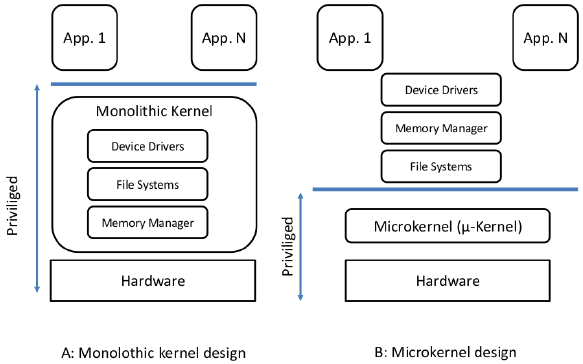
\includegraphics[width=\textwidth]{pictures/mono-micro_kernels.png}
  \caption{Α.Μονολιθική και \en{Microkernel} αρχιτεκτονική πυρήνα}
  \label{fig:microkernels}
\end{figure}

Το σκεπτικό πίσω από τον όρο \en{anykernel} επεκτείνει περαιτέρω τον ανώτερο διαχωρισμό
των λειτουριών ενός συστήματος που παραδοσιακά επιτελούνται εντός του πυρηνα.
Πλέον, οι \en{drivers} του συστήματος
ανεξαρτητοποιούνται από το σύστημα στο οποίο εν τέλει θα
εκτελεστούν. Αναφερόμαστε σε μια αρχιτεκτονικά αγνωστική
προσέγγιση, όπου οι \en{drivers} μπορούν είτε να ενσωματώνονται
σε κάποιο μονολιθικό πυρήνα, σε κάποιο \en{microkernel}, σε
κάποιο \en{exokernel}, γενικά σε πυρήνες διαφορετικών αρχιτεκτονικών,
ή να εκτελούνται ως διεργασία στο \en{user space} χωρίς κάποια
αλλαγή στον κώδικά τους. Ως \en{drivers} δεν εννοούμε μόνο τους
οδηγούς συσκευών, αλλά και το σύστημα αρχείων, την στοίβα
δικτύου κ.α.. Υπάρχει, λοιπόν, μια εγγενής φορητότητα των
\en{drivers}\cite{noOSnoProb}. Το λειτουργικό σύστημα \en{NetBSD} ταιριάζει στον
ορισμό του \en{anykernel}\cite{interviewKantee}.
\newline

Σχετική έννοια είναι αυτή των \en{rump kernels}. Με τον όρο \en{rump }
εννοούμε ένα κατάλοιπο ενός μεγαλύτερου αρχικού συνόλου.
\en{Rump kernel}, λοιπόν, είναι ένα εικονικοποιημένο στιγμιότυπο
ενός συνόλου από \en{drivers}, οι οποίοι τρέχουν εκτός του
μονολιθικού πυρήνα. Αυτό πρακτικά μεταφράζεται σε έναν
πυρήνα ενός παραδοσιακού λειτουργικού συστήματος, από
το οποίο έχουν αφαιρεθεί διάφορα κομμάτια, όπως η εικονική
μνήμη και ο συγχρονισμός μεταξύ διεργασιών. Το υπόλειμμα
(\en{rump}) είναι οι \en{drivers} και οι απολύτως απαραίτητες ρουτίνες, ώστε
να μπορεί να εκτελεστεί μία διεργασία\cite{Orestis}. Μπορούμε να φανταστούμε
τους \en{rump kernels} σαν πυρήνας-ως-υπηρεσία (\en{kernel-as-a-service}).
Οι \en{rump kernels} που δημιουργήθηκαν από τον \en{Antii Kantee}
εξάγουν τους \en{drivers} και τα στοιχεία από το λειτουργικό σύστημα
\en{NetBSD}, δηλαδή από τον \en{open-source} πηγαίο κώδικά του\cite{interviewKantee}.
\newline

Το \en{rumprum unikernel} είναι μια εφαρμογή των \en{rump kernels}, που
έχει στόχο να εκτελούνται προγράμματα ως \en{unikernel}. Υπενθυμίζεται
ότι ο αρχικός στόχος του εγχειρήματος των \en{rump kernel} ήταν
να εκτελούνται αυτόνομα \en{drivers} στο \en{user space}, ώστε να
διευκολύνεται η ανάπτυξη και η αποσφαλμάτωσή του. Όμως, με
την πάροδο του χρόνου, αποδείχθηκε πως οι \en{rump kernels} μπορούν
να εκτελεστούν ως εικονικοποιημένος \en{guests} επάνω στον \en{Xen hypervisor}.
Η πρώτη εφαρμογή αυτού του «παντρέματος» ήταν η εκτέλεση ελαφρών
\en{router} ή \en{firewalls} ως \en{guests}, λειτουργίες που παραδοσιακά
βρίσκονταν στον χώρο ενός μονολιθικού πυρήνα. Σύντομα προστέθηκε
και η ύπαρξη μια διεπαφής από τον χώρο χρήστη, δηλαδή ένας
τρόπος να καλούνται οι κλήσεις συστήματος\cite{RumprunXen}. Με όλα αυτά τα
επίπεδα λογισμικού διαθέσιμα, είναι προφανές ότι οι \en{rump kernels}
έχουν την δυνατότητα να παράγουν \en{unikernels}, τα οποία ονομάστηκαν
\en{Rumprun unikernels}. Η σχέση μεταξύ του \en{Rumprun} και των \en{rump kernels},
είναι πως για την ανάπτυξη του \en{unikernels}, το \en{Rumprun} επιλέγει
από το σύνολο που προσφέρουν οι \en{rump kernels} μόνο τα στοιχεία
που είναι απαραίτητα για την εκτέλεση μιας συγκεκριμένης εφαρμογής,
το οποίο σημαίνει πως το \en{Rumprun} είναι μια από τις πολλές
εφαρμογές (\en{use cases}) των \en{rump kernels}. Η εικόνα \ref{fig:any_rumpk_Rumprun}
παρουσιάζει καλύτερα την σχέση μεταξύ του \en{anykernel} των \en{rump kernels}
και του \en{Rumprun unikernel}.
\newline

\begin{figure}[h]
  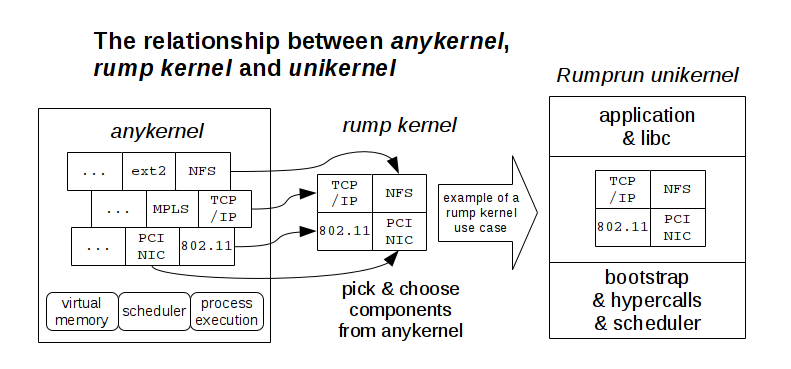
\includegraphics[width=\textwidth]{pictures/anykernel-rumpkernel.PNG}
  \caption{Σχέση μεταξύ \en{anykernel-rump kernels-Rumprun}}
  \label{fig:any_rumpk_Rumprun}
\end{figure}


\subsubsection{Δομή και Ανάπτυξη του \en{Unikernel}}

Η στοίβα λογισμικού του \en{Rumprun}, θυμίζει σε ένα βαθμό την στοίβα
εκτέλεσης μιας διεργασίας σε κάποιο συμβατικό λειτουργικό
σύστημα. Στο ανώτερο επίπεδο βρίσκεται ο κώδικας της εφαρμογής,
ο οποίος στηρίζεται σε βιβλιοθήκες του \en{user space}, όπως π.χ. η \en{libc}
για την γλώσσα \en{C}. Από κάτω βρίσκονται οι κώδικας που αναλαμβάνει
να καλέσεις τις κλήσεις συστήματος (\en{system calls}) προς τον
πυρήνα. Μια διαφορά που υπάρχει στο \en{Rumprun} είναι πως οι κλήσεις
αυτές δεν γίνονται με
κάποια \en{trap} εντολή ώστε να αλλάξει το επίπεδο προνομίων με το
οποίο εκτελείται ο κώδικας, αλλα καλείται απλά μια απλή συνάρτηση
βιβλιοθήκης η οποία αναλαμβάνει να εξυπηρετήσει την αίτηση.
Υπενθυμίζεται πως σε \en{unikernel} όλη η εκτέλεση γίνεται σε ένα
μοναδικό ενιαίο χώρο μνήμης, δεν υπάρχει διάκριση μεταξύ
\en{user space} και \en{kernel space}. Για να το πετύχει αυτό, το
\en{Rumprun} αντικαθιστά όλες τις κλήσεις συστήματος (\en{system calls})
του \en{NetBSD} δικές του κλήσεις πυρήνα (\en{rump kernel calls}), οι
οποίες είναι στην ουσία κλήσεις συναρτήσεων (\en{library calls}).
Από αυτό το επίπεδο και μέχρι το επίπεδο του επόπτη βρίσκεται
ό,τι θα έπρεπε να βρίσκεται στον πυρήνα ενός συμβατικού λειτουργικού.
\newline

Εύλογα θα περίμενε κανείς, στα κατώτερα επίπεδα να βρίσκονται
κομμάτια λογισμικού μόνο από τους \en{rump kernels}. Εντούτοις,
οι \en{rump kernels} δεν σχεδιάστηκαν ώστε να τρέχουν επάνω σε κάποιο
επόπτη ως εικονική μηχανή, οπότε τους λείπει η δυνατότητα να
επικοινωνούν με το χαμηλότερο επίπεδο του επόπτη. Ταυτόχρονα
απουσιάζουν και οι μέθοδοι εκκίνησης (\en{bootstrap}), χρονοδρομολόγησης,
διακοπές (\en{interrupt}), και διαχείριση των σελίδων της μνήμης.
Για αυτόν ακριβώς τον λόγο, στον στοίβα του \en{Rumprun} κάτω
από το κομμάτι των \en{rump kernels} έχει προστεθεί ένα στρώμα
υλικού που ονομάζεται \en{Bare Metal Kernel (bmk)}, και που
ρόλος του είναι να επιτελεί όλες αυτές τις σημαντικότατες
ανώτερες λειτουργίες.
Ο \en{bmk} αποτελείται τόσο από κώδικα
που είναι κοινός για κάθε πλατφόρμα στην οποία στοχεύει το
\en{Rumprun}, όσο και από κώδικα ειδικό για κάθε πλατφόρμα
ξεχωριστά\cite{Orestis}. Παράλληλα, υπάρχει και ένας μηχανισμός
επικοινωνίας των \en{rump kernels} με τον \en{bmk}, που ονομάζεται
\en{rumpuser}\cite{noOSnoProb}. Οι βασικοί στόχοι του \en{Rumprun} είναι είτε ο \en{Xen hypervisor},
είτε το \en{KVM} των \en{Linux}, είτε απευθείας το υλικό (\en{bare metal}).
\newline

Η δομή της στοίβας φαίνεται στην εικόνα \ref{fig:RumprunStack}
\newline
\begin{figure}[h]
  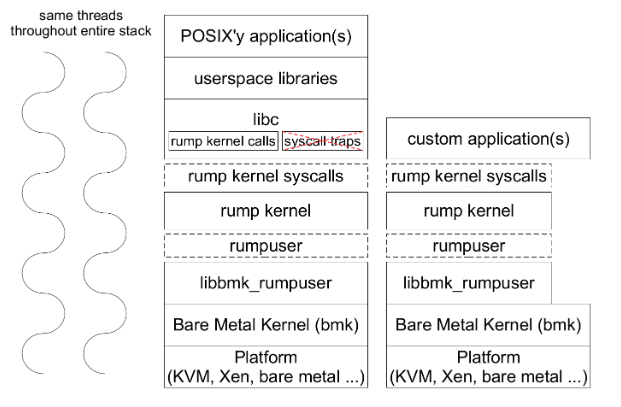
\includegraphics[width=\textwidth]{pictures/rumprun-stack.PNG}
  \caption{Στοίβα λογισμικού \en{rump kernels/Rumprun}}
  \label{fig:RumprunStack}
\end{figure}


Αξίζει, επίσης, να περιγραφεί η διαδικασία ανάπτυξης ενός \en{unikernel} με
το \en{Rumprun framework}. Η διαδικασία αποτελείται χονδρικώς από τέσσερα βήματα.
\begin{enumerate}
  \item Αρχικά αναπτύσσεται ο κώδικας της εφαρμογής σε
  \en{userspace}. Το \en{Rumprun} στοχεύει στην εκτέλεση \en{POSIX }
  εφαρμογές, οπότε η ανάπτυξη δεν διαφέρει από συμβατικά
  λειτουργικά, και συνήθως μπορεί να χρησιμοποιηθεί κώδικας
  από εφαρμογές ήδη γραμμένες για κάποια άλλη πλατφόρμα,
  όπως το \en{linux}. Ωστόσο, συγκεκριμένες λειτουργίες, όπως οι
  πολλές διεργασίες και η εικονική μνήμη δεν υποστηρίζονται,
  άρα εφαρμογές που στηρίζονται σε κλήσεις όπως \en{fork()} ή
  η \en{mmap()} πρέπει να προσαρμόζονται.

  \item Στην συνέχεια ο κώδικας γίνεται \en{compiled} σε
  ένα ή περισσότερα \en{object file}, όπως κατά συμβατικές
  διαδικασίες μεταγλώττισης. Το \en{Rumprun} στηρίζεται σε
  \en{cross-compilation}, όποτε δεν υπάρχει ανάγκη ύπαρξης
  κάποιου \en{unikernel} το οποίο μπορεί να μεταγλωτίζει, αλλά
  αντί αυτού προσφέρονται έτοιμοι \en{compilers}.

  \item Έπειτα έρχεται η σειρά του \en{linking} αυτών των
  αντικειμένων. Δεν πρόκειται για συμβατικό \en{linking},
  αλλά για \en{pseudo-linking}, καθώς οι εξαρτήσεις από το
  λειτουργικό σύστημα, για παράδειγμα οι κλήσεις συστήματος,
  δεν γίνονται \en{resolve} αλλά γίνεται μόνο έλεγχος για την
  ορθή συντακτική χρήση τους. Δεν επιτελείται, συνεπώς,
  κάποια σύνδεση με τα συστατικά του λειτουργικού συστήματος,
  που σε άλλη περίπτωση θα επέτρεπαν την επικοινωνίας κατά το
  \en{runtime}. Σε αυτή την φάση, παράγεται ένα αρχείο το οποίο
  θυμίζει εκτελέσιμο, όμως δεν είναι.

  \item Τέλος, επέρχεται το λεγόμενο \en{bake}, δηλαδή οι
  προαναφερθείσες εξαρτήσεις συνδέονται με τις συναρτήσεις
  των \en{rump kernels} που αναλαμβάνουν τις λειτουργίες που
  ζητούνται. Από το σύνολο των \en{drivers} των \en{rump kernels} εξάγονται
  μόνο όσοι χρειάζονται πραγματικά από την εφαρμογή. Ταυτόχρονα,
  προστίθεται και τα κομμάτια που χρειάζονται για την επικοινωνία
  με τον επόπτη στον οποίο στοχεύουμε.
\end{enumerate}
Με αυτόν τον τρόπο παράγεται το τελικό \en{unikernel}, η μικρή, ασφαλής
και γρήγορη εικονική μηχανή, που θα επιτελεί την λειτουργία για την
οποία σχεδιάστηκε.

\subsubsection{Γιατί \en{Rumprun}}

Όπως αναφέρθηκε, επιλέγεται το \en{Rumprun} να είναι το \en{framework}
επάνω στο οποίο εργαζόμαστε για την υλοποίηση της παρούσας
εργασίας. Θυμίζεται πως επιθυμείται να ενσωματώθει η λειτουργία
ελαστικής μνήμης \en{utmem}, η οποία αναλύεται αναλυτικότερα στην
συνέχεια, σε κάποιο \en{unikernel framework}. Το \en{rump kernels - Rumprun}
επιλέχθηκε ως κατάλληλο εργαλείο για τους εξής λόγους:

\begin{itemize}
  \item Ο μηχανισμός \en{utmem}, τουλάχιστον για το \en{frontend }
  που χρειάζεται να υλοποιηθεί από την αρχή, είναι ουσιαστικά ένας \en{driver}
  που επικοινωνεί με τον \en{hypervisor}. Αφού, λοιπόν, τα \en{rump kernels }
  επιτρέπουν την εξαγωγή \en{drivers} γραμμένους για το \en{NetBSD}, ένα
  \en{well-documented} λειτουργικό σύστημα, είναι εύλογο να ταιριάζουν
  στο \en{use case} μας και να διευκολύνουν το έργο μας.

  \item Το \en{Rumprun} στοχεύει στο να υποστηρίζει την
  μετατροπή των περισσότερων εφαρμογών οι οποίες υπακούν στο
   \en{POSIX} πρότυπο σε \en{unikernel}. Συνέπεια αυτού είναι πως δεν
   χρειάζεται ιδιαίτερη προσαρμογή επιλογών για να αναπτυχθεί \en{user space}
   κώδικα που να χρησιμοποιεί την \en{utmem}, καθώς η συντριπτική πλειοψηφία των
   προγραμματιστών γνωρίζει το \en{POSIX} πρότυπο,

  \item Στην στοίβα του \en{Rumprun} απουσιάζει από
  επιλογή των σχεδιαστών η εικονική μνήμη. Αυτή η επιλογή
  έγινε για να είναι όσο το δυνατόν ελαφρύτερα και απλούστερα
  τα τελικά \en{unikernel}. Ως εκ τούτου, το να ενσωματωθεί ο
  μηχανισμός της \en{utmem} σε ένα τέτοιο \en{unikernel framework},
  στην πράξη προσφέρει λύση σε ένα υπαρκτό ενδεχόμενο,
  δηλαδή στην διαχείριση περιορισμένης μνήμης. Η συγκεκριμένη εργασία
  επικεντρώνεται στην αντιμετώπιση αυτού του προβλήματος. Όπως θα
  φανεί και στην συνέχεια, πράγματι έχει ουσιαστική αξία η
  υλοποίηση της εργασίας.

\end{itemize}







\section{Μνήμη - \en{utmem}}

\subsection{Ιστορία}

Η διαχείριση της μνήμης ενός υπολογιστικού συστήματος είναι ένα
πολύ σημαντικό πρόβλημα που καλείται να λύσει o μηχανικός
υπολογιστικών συστημάτων. Η μνήμη αποτελεί σημαντικότατο πόρο, αν όχι τον σημαντικότερο.
Στα συμβατικά λειτουργικά συστήματα, κάθε διεργασία που εκτελείται
νομίζει πως βρίσκεται σε ένα ενιαίο χώρο μνήμης, τον οποίον
δεν μοιράζεται με άλλες εργασίες, οι οποίες μπορεί να βρίσκονται
στο σύστημα την στιγμή της εκτέλεσης. Το λειτουργικό σύστημα
από την άλλη, οφείλει να αντιστοιχεί αυτόν τον χώρο διευθύνσεων
που «βλέπει» η διεργασία (\en{virtual address space}), σε κάποιο κομμάτι της
φυσικής μνήμης του συστήματος (\en{physical address space}),
χρησιμοποιώντας μηχανισμούς και πολιτικές τόσο σε επίπεδο υλικού όσο και λογισμικού.
\newline

Πρόβλημα εμφανίζεται όταν η φυσική μνήμη του συστήματος γεμίσει
από εγγραφές και πλέον το λειτουργικό αδυνατεί να κατανείμει
περισσότερη στα προγράμματα. Αν δεν αντιμετωπιστεί αυτό το
πρόβλημα, και απλά αρνηθεί το λειτουργικό σύστημα να δώσει νέα
μνήμη, τότε προκύπτει ένα ασταθές, δυσλειτουργικό και
αναποτελεσματικό σύστημα. Η λύση, που πλέον ενσωματώνεται σε όλα
τα σύγχρονα λειτουργικά συστήματα όπως \en{Linux, Windows} κλπ, είναι
η ύπαρξη της εικονικής μνήμης (\en{virtual memory}), δηλαδή ενός
μηχανισμού που επιτρέπει στο σύστημα να δίνει στα προγράμματα την ψευδαίσθηση
πως υπάρχει περισσότερη διαθέσιμη μνήμη από την φυσική. Όταν η
μνήμη γεμίσει, σελίδες (\en{memory pages}) αυτής εναλλάσσονται (\en{swapping})
σε κάποιο άλλο αποθηκευτικό μέσο, διαθέσιμο στο σύστημα, το οποίο
συνήθως είναι κάποιος δίσκος. Όταν χρειαστεί να προσπελαστούν οι
σελίδες που έχουν μεταφερθεί στον δίσκο τότε αντιγράφονται πίσω
στην κύρια μνήμη, στην θέση κάποιων άλλων οι οποίες με την σειρά
του θα μετακινηθούν στον δίσκο. Οι αποθηκευτικοί δίσκοι έχουν
χωρητικότητα αρκετές φορές μεγαλύτερη από της φυσικής μνήμης,
έτσι λοιπόν επιτυγχάνεται η ψευδαίσθηση της περισσότερης
διαθέσιμης μνήμης\cite{wikiVirtMemory}. Το μεγάλο μειονέκτημα αυτής της τεχνικής
είναι πως, επειδή η ταχύτητα ανάγνωσης και εγγραφής του δίσκου
είναι τάξης μεγέθους πιο αργή από της φυσικής μνήμης, η επίδοση
και ταχύτητα εκτέλεσης των προγραμμάτων μειώνεται δραματικά. Για
εφαρμογές που μας ενδιαφέρει η υψηλή ταχύτητα εκτέλεσης και χαμηλή
 καθυστέρηση, όπως π.χ. μια διαδικτυακή εφαρμογή που προσφέρει
 περιεχόμενο σε πελάτες, αυτό είναι καταστροφικό.
\newline

Σε περιβάλλον εικονοποίησης και ειδικά σε \en{cloud virtualization},
το ανώτερο πρόβλημα γίνεται ακόμα πιο σύνθετο. Ένα λειτουργικό
που εκτελείται ως \en{guest}, αγνοεί το πραγματικό μέγεθος της φυσικής
μνήμης του μηχανήματος επάνω στο οποίο εκτελείται, με αποτέλεσμα
σε αρκετές περιπτώσεις αυτή να υποχρησιμοποιείται. Επίσης, και ο
\en{host} αγνοεί την οποιαδήποτε ύπαρξη μηχανισμών διαχείρισης της
μνήμης από τον \en{guest}\cite{paperAimiliou}. Έστω το εξής σενάριο παράλληλης εικονικοποίησης
δύο \en{guest} λειτουργικών συστημάτων επάνω στο ίδιο μηχάνημα: ο πρώτος
\en{guest} έχει εξαντλήσει όλη την μνήμη η οποία του έχει ανατεθεί, και
άρα έχει οδηγηθεί σε λιγότερο αποδοτικές λύσεις όπως το \en{swapping},
ενώ o δεύτερος έχει ακόμα ένα μεγάλο ποσοστό της μνήμης του
ελεύθερο. Έτσι, παρόλο που η συνολική μνήμη θεωρητικά αρκεί για
τις ανάγκες όλων, εντούτοις δεν χρησιμοποιείται σωστά.
\newline

Έχουν προταθεί διάφοροι τρόποι αντιμετώπισης αυτού του γενικού προβλήματος, οι οποιοι συνοψίζονται σε
\begin{enumerate}
  \item Υπερανάθεση πόρων (\en{Overprovisioning}). Σε αυτήν την περίπτωση
  οι σχεδιαστές δρουν σκεπτόμενοι πάντα το χειρότερο δυνατό σενάριο. Δηλαδή,
  αναθέτουν στους \en{guests} αρκετή μνήμη ώστε πρακτικά να εξαλείφεται
  το ενδεχόμενο να μην του αρκέσει και να στραφούν στην εικονική
  μνήμη. Το μεγάλο μειονέκτημα, είναι πως πρώτον χρειαζόμαστε να
  υπάρχει διαθέσιμη ως φυσική μνήμη όλη αυτή που παραχωρείται,
  οπότε μπορούν να υποστηριχθούν λιγότεροι \en{guests} ανά μονάδα
  μνήμης, και δεύτερον πως προφανώς ο πόρος της μνήμης πάλι υποχρησιμοποιείται.

  \item Εναλλαγή στον δίσκο (\en{swapping}). Αυτό είναι ή άλλη όψη του
  νομίσματος, δηλαδή να επιτρέπεται οι \en{guests} να χρησιμοποιούν την
  εικονική τους μνήμη σε περίπτωση που τελειώσει η διαθέσιμή του. Μειώνεται η μνήμη που
  ανατίθεται σε κάθε guests, αδιαφορώντας για πιθανούς εσωτερικούς μηχανισμούς διαχείρισής της.
  Μπορούν να υποστηριχθούν περισσότεροι \en{guests} ανά μονάδα μνήμης,
  αλλά η επίδοση κάποιων εξ αυτών χάνεται.

  \item \en{Ballooning}. Η πιο ισορροπημένη και δημοφιλής μέθοδος.
  Ουσιαστικά αυξομειώνεται δυναμικά η διαθέσιμη μνήμη του \en{guest}
  κατά το \en{runtime}, ανάλογα με τις ανάγκες του. Για να λειτουργήσει
  το \en{ballooning} πρέπει \en{host} και \en{guest} να συνεργαστούν, δηλαδή
  αποτελεί εφαρμογή του \en{paravirtualization}. Αρχικά, τονίζεται πως
   \en{host} και \en{guest} «βλέπουν» διαφορετικά την μνήμη. Ο \en{guest} νομίζει
   πως διαχειρίζεται διευθύνσεις φυσικής μνήμης, όπως αν
   εκτελούνταν απευθείας επάνω στο υλικό, όμως στην ουσία αποτελεί
   μια διεργασία του \en{host} λειτουργικού, ή πιο γενικά του
   \en{hypervisor}. Άρα οι διευθύνσεις του είναι ουσιαστικά εικονικές,
   τις οποίες οφείλει ο \en{host} να αντιστοιχεί σε φυσική μνήμη.
   Με το \en{ballooning}, ο \en{guest} εναποθέτει τις σελίδες μνήμης
   (\en{memory pages}) του τις οποίες δεν χρησιμοποιεί σε μια ειδική
   συσκευή στον πυρήνα του λειτουργικού συστήματος, σαν να
   δηλώνει πως παραιτείται από την κυριότητά του επάνω σε αυτές.
   Με την σειρά της, η συσκευή επικοινωνεί  με τον \en{hypervisor},
   ο οποίος πλέον γνωρίζει πως δεν χρειάζεται να αντιστοιχεί
   αυτές τις εικονικές διευθύνσεις μνήμης που το έδωσε ο \en{guest}
   σε φυσική μνήμη, και άρα η πλέον απελευθερωμένη μνήμη μπορεί
   να χρησιμοποιηθεί για άλλο σκοπό, και όχι να περιμένει
   ανενεργή. Όταν πάλι ο \en{guest} χρειαστεί περισσότερη μνήμη,
   δηλώνει στην συσκευή πως ξαναπαίρνει την κυριότητα αυτών
   των σελίδων, οπότε με την σειρά του ο \en{host} αντιστοιχεί
   πάλι φυσική μνήμη σε αυτές τις σελίδες. Το μειονέκτημα
   της συγκεκριμένης τεχνικής πηγάζει από το γεγονός πως τα σύγχρονα λειτουργικά συστήματα είναι σχεδιασμένα
   ώστε να χρησιμοποιούν όλη την διαθέσιμη μνήμη του συστήματος,
   θεωρώντας πως είναι η μόνη οντότητα που έχει ανάγκη από
   την υφιστάμενη φυσική μνήμη. Για παράδειγμα, το \en{page cache}
   υποσύστημα στο \en{linux}, αντιστοιχεί σελίδες δεδομένων του
   δίσκου σε αχρησιμοποίητες από διεργασίες σελίδες της κύριας
   μνήμης, Έτσι ένας \en{guest} δεν έχει λόγο να αποδεσμεύσει τις
   σελίδες του χρησιμοποιώντας την συσκευή \en{ballooning}.
   Προκύπτει, λοιπόν, αυτομάτως μια σχέση ανταγωνισμού, και όχι συνεργασίας
   για την μνήμη ανάμεσα στον \en{host} και τον \en{guest}\cite{paperAimiliou}.


\end{enumerate}




%TMEM
\subsection{\en{Transcedent memory - tmem}}

Μια διαφορετική λύση, στο πρόβλημα της διαχείρισης της μνήμης σε
\en{virtualized} περιβάλλοντα, είναι αυτή της μεταβατικής (πτητικής) μνήμης
(\en{transcendent memory} ή \en{tmem}). Η \en{tmem} πρόκειται για να \en{linux kernel module}
το οποίο αναπτύχθηκε από την εταιρία \en{Oracle} το 2009, για
τον \en{Xen hypervisor}, και ενσωματώθηκε στον πυρήνα του \en{linux}, σχεδόν άμεσα\cite{tmemXenSummit}.
\newline

Η βασική φιλοσοφία πίσω από την ιδέα αυτή, είναι να ανταλλάσσεται
μνήμη, ή μάλλον δεδομένα, μεταξύ \en{guest} και \en{host} χρησιμοποιώντας μια βάση
δεδομένων η οποία λειτουργεί με πρότυπο αναφοράς κλειδιού-τιμής
(\en{key-value})\cite{Aimilios}. Τα δεδομένα σε αυτήν την βάση θα είναι
σελίδες μνήμης του \en{guest}, όχι κενές αλλά με εγγραφές εντός αυτών. Διαφέρει με την τεχνική του
\en{ballooning}, στο γεγονός πως η μνήμη που ανατίθεται με την \en{tmem}
δεν είναι προσπελάσιμη απλά με αναφορά σε κάποια διεύθυνση
μνήμης με κάποιο απλό \en{load-store}. Η πρόσβαση στην μνήμη αυτή,
γίνεται μόνο μέσω ειδικών κλήσεων επόπτη (\en{hypercalls}),
χρησιμοποιώντας το κατάλληλο κλειδί κάθε φορά. Αυτό, εκ πρώτης,
ακούγεται αποθαρρυντικό, ίσως και λάθος σχεδιαστικά, όμως επιτρέπει
μεγαλύτερη ευελιξία στην μορφή που εν τέλει αποθηκεύονται τα
δεδομένα. O \en{host}, ή εν γένει οποιοδήποτε σύστημα καλείται να
αποθηκεύσει την μνήμη αυτή, μπορεί να την μετασχηματίσει, να
την τροποποιήσει και να την μεταφέρει οπουδήποτε κρίνει
αυτός κατάλληλο, εφόσον δεσμεύεται πως μπορεί να την ανακτήσει
και να την επιστρέψει πίσω στον \en{guest}, όταν και αν αυτός το ζητήσει\cite{tmemNutshell}.
\newline

Η μηχανισμός της \en{tmem}, ακουλουθεί μια απλή και προσεκτικά
σχεδιασμένη διεπαφή, ικανή να καλύψει ένα ευρύ φάσμα
περιπτώσεων. Η διεπαφή αυτή έχει σχεδιαστεί με γνώμονα να
είναι ευέλικτη και να έχει ελάχιστο αποτύπωμα και κόστος
στον πυρήνα που την χρησιμοποιεί. Όπως αναφέρθηκε, η \en{tmem}
δεν είναι άμεσα προσπελάσιμη από τον \en{guest}, αλλά έμμεσα μέσα
από ειδικές αιτήσεις στον επόπτη , ή εν γένει σε όποιον την
διαχειρίζεται. Δημιουργείται στην αρχή μια δεξαμενή μνήμης
(\en{pool}), με ξεχωριστό \en{pool id}. Επίσης, δημιουργούνται μοναδικά
κλειδιά (\en{handles}), τα οποία αποτελούν αντίστοιχο ρόλο με τις
διευθύνσεις των σελίδων μια συμβατικής μνήμης. Τα κλειδιά αυτά
είναι μοναδικά για κάθε κομμάτι μνήμης που αποθηκεύεται στο
\en{pool}, αλλά όχι μεταξύ διαφορετικών \en{pools}. Οι βασικές ενέργειες
επάνω στην \en{tmem} είναι η λήψη (\en{Get}) και η τοποθέτηση (\en{Put}).
Όταν ο \en{guest}, επιθυμεί να αποθηκεύσει δεδομένα τότε εκτελεί μια
αίτηση \en{Put} στον \en{hypervisor}, αναφέροντας το σωστό \en{pool id} και
τα σωστά κλειδιά, καθώς και την περιοχή μνήμης του στην οποία βρίσκονται
τα δεδομένα που θέλει να αποθηκευτούν\cite{tmemXenSummit}. Αντίστοιχα, όταν
θέλει να ανακτήσει τα δεδομένα, εκτελεί μια αίτηση \en{Get}, με
τις αντίστοιχες παραμέτρους. Η μηχανισμός \en{tmem}, σε αντίθεση
με I/O μηχανισμούς, είναι σύγχρονος όσον αφορά την αντιγραφή
των δεδομένων, και ως εκ τούτου προκύπτει η ανάγκη ύπαρξης
δικλείδων ασφαλείας για να αποφεύγονται \en{deadlocks}\cite{tmemNutshell}.
\newline

Όπως φαίνεται μέχρι στιγμής, η μηχανισμός \en{tmem} στηρίζεται
στην επικοινωνία δύο μορφών χρηστών, μεταξύ δηλαδή του
\en{frontend}, δηλαδή του μηχανισμού-χρήστη που επιθυμεί να αποθηκεύει
κομμάτια μνήμης του, και του \en{backend}, δηλαδή του μηχανισμού-χρήστη ο
οποίος αναλαμβάνει την αποθήκευση. Μηχανισμοί \en{backend} μπορούν να
είναι διάφοροι, ενδεικτικά:

\begin{enumerate}
  \item \en{Transcendent memory for Xen}. Ο \en{Xen hypervisor} ήταν
  ο αρχικός στόχος του εγχειρήματος, οπότε είναι ο πιο
  ώριμος από τα \en{backend}. Αποθηκεύει στην μνήμη του \en{hypervisor }
  τα δεδομένα, ενώ υποστηρίζει πολλαπλούς \en{guests}, συμπίεση
  και μοναδική αποθήκευση διπλότυπων δεδομένων, αν εμφανίζονται
  από διαφορετικούς \en{guests}, για εξοικονόμηση χώρου

  \item \en{Zcache}. Η \en{Zcache} επιτρέπει την αποθήκευση πολλαπλάσιων
  σελίδων μνήμης μέσω της \en{tmem} όταν η μνήμη δεν είναι διαθέσιμη.
  Το καταφέρνει αυτό χρησιμοποιώντας συμπίεση δεδομένων μέσα
  στον πυρήνα. Δεν αφορά απαραίτητα κάποιον \en{hypervisor}, αφού η
  ανταλλαγή δεδομένων μπορεί να γίνεται ανάμεσα σε δύο μέρη του ίδιου ίδιου
  πυρήνα, οδηγεί όμως σε καλύτερη αξιοποίηση των πόρων\cite{tmemNutshell}.

\end{enumerate}

Μεγαλύτερο ενδιαφέρον παρουσιάζουν οι χρήστες \en{frontend}, δηλαδή
ποια συστήματα ενός λειτουργικού συστήματος αξίζει να χρησιμοποιούν
την \en{tmem}. Αυτά είναι:

\begin{enumerate}
  \item Το \en{frontswap subsystem}. Η λειτουργία του στον πυρήνα του
  \en{linux} είναι να εναλλάσσει (\en{swap}) σελίδες μνήμης από την κύρια
  μνήμη σε κάποιο δευτερεύον αποθηκευτικό μέσο. Χρησιμοποιεί μόνιμα
  σύνολα, που σημαίνει για οποιοδήποτε σελίδα μνήμης αποθηκευτεί
  στο \en{frontswap}, υπάρχει εγγύηση πως θα βρίσκεται εκεί ανά πάσα
  στιγμή το αναζητήσει πίσω αυτός που το τοποθέτησε. Ως χρήστης
  του \en{tmem} μηχανισμού, το \en{frontswap} επιλέγει να προωθεί τις σελίδες
  μνήμης στα \en{backend} της \en{tmem}, και να μην τις στέλνει απευθείας στο
  δίσκο που είναι τάξης μεγέθους πιο αργός από την κύρια μνήμη.
  Υπάρχει, βέβαια, πάντα το ενδεχόμενο το \en{backend} να απορρίψει την
  αίτηση \en{tmem} για διάφορους λόγους που επιλέγει το ίδιο, και τότε
  να πρέπει το \en{frontswap} να καταφύγει στον δίσκο. Γενικώς, επιτυγχάνεται
  αυξημένη ταχύτητα πρόσβασης στις σελίδες οι οποίες δίνονται στο \en{frontswap}
  από την κύρια μνήμη.

  \item Το \en{cleancache subsystem}. Κατά την εκτέλεση των προγραμμάτων,
  είναι πολύ συχνό να μεταφέρονται δεδομένα από τον δίσκο στην κύρια
  μνήμη και τούμπαλιν. Στο \en{Linux}, η πρόσβαση στις συσκευές και άρα
  και στον δίσκο γίνεται μόνο μέσα από έγκριση του πυρήνα, και καμία
  διεργασία δεν μπορεί να τις χρησιμοποιήσει απευθείας. Έτσι, αυτές οι
  συναλλαγές περνάν από τον πυρήνα πρώτα. Η \en{cleancache} συμπεριφέρεται
  κατά αντιστοιχία με την \en{cache} στις \en{CPUs}, αλλά αντί να διατηρεί εφήμερα
  δεδομένα ανάμεσα στον επεξεργαστή και την κύρια μνήμη, διατηρεί σελίδες
  δεδομένων ανάμεσα στην μνήμη και στον δίσκο. Θυμίζεται πως αυτά τα
  δεδομένα βρίσκονται και ως αντίγραφα σε άλλες θέσεις, είτε στον δίσκο
  είτε στην μνήμη, και πως είναι και εφήμερα, που σημαίνει πως μπορεί στην θέση
  του να γραφτούν άλλα και άρα δεν υπάρχει εγγύηση για την ύπαρξη τους
  ανά πάσα στιγμή. Με την \en{tmem}, αυτά τα δεδομένα μπορούν να αποθηκευτούν
  σε κάποιο \en{tmem pool}, και άρα η απουσία τους από τη \en{cleancache} να μην
  οδηγεί απαραίτητα σε ανάκτηση (\en{fetch}) από τον δίσκο, που είναι και αρκετά
  αργή διαδικασία\cite{Aimilios}.
\end{enumerate}

\begin{figure}[h]
  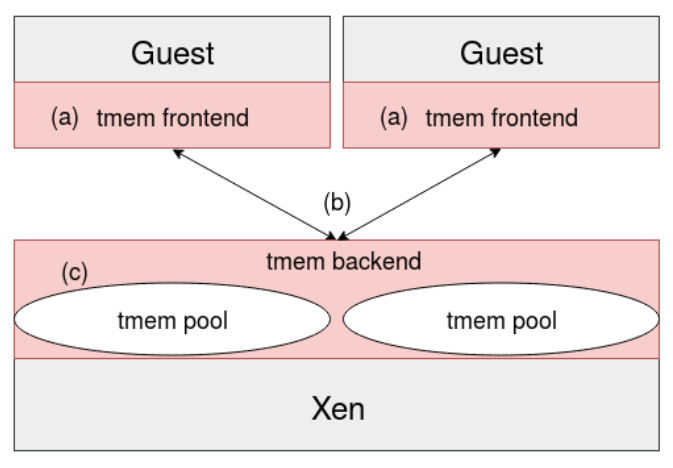
\includegraphics[width=0.5\textwidth]{pictures/tmemXen.PNG}
  \caption{\en{Tmem} επάνω στον \en{Xen hypervisor}}
  \label{fig:tmemXen}
\end{figure}






%UTMEM

\subsection{\en{Userspace transcedent memory - utmem}}

Μέχρι στιγμής ο μηχανισμός \en{tmem}, αφορά περιπτώσεις χρήσης από
υποσυστήματα που τρέχουν «σιωπηλά» εντός του πυρήνα. Ένας
προγραμματιστής, όχι μόνο αγνοεί την ύπαρξη ενός τέτοιου συστήματος,
αλλά ούτε είναι σε θέση να αναπτύξει προγράμματα ικανά να χρησιμοπούν ρητά τον μηχανισμό.
Δημιουργείται, συνεπώς, η
εύλογη απορία αν θα ήταν δυνατόν ένας τέτοιος μηχανισμός να
είναι διαθέσιμος στο \en{user space}.
\newline

Η απάντηση δόθηκε σε μια προηγούμενη διπλωματική εργασία του εργαστηρίου
υπολογιστικών συστημάτων του Εθνικού Μετσοβίου Πολυτεχνείου,
 όπου υλοποιήθηκε ένας τέτοιος μηχανισμός από τον Αιμίλιο Τσαλαπάτη.
Ονομάστηκε \en{utmem} (από το \en{user space tmem}). Αποδείχθηκε,
μάλιστα, πειραματικά πως σε συγκεκριμένες περιπτώσεις πίεσης
μνήμης οι διεργασίες που χρησιμοποιούν αυτόν τον μηχανισμό \en{utmem}
συμπεριφέρονται καλύτερα από διεργασίες που στηρίζονται σε
\en{tmem} μόνο έμμεσα με χρήση του \en{frontswap subsystem}\cite{Aimilios}\cite{paperAimiliou}.
\newline

Η δομή του μηχανισμούς είναι πολύ απλή, και αφορά την επικοινωνία ενός \en{linux guest},
ο οποίος τρέχει επάνω στο \en{KVM}, και ενός \en{linux host}. Αυτή τη
στιγμή, η \en{utmem} συνεργάζεται μόνο με το \en{KVM} ως \en{hypervisor}.
\newline

Αρχικά σχεδιάστηκε μια εικονική συσκευή (\en{virtual device}), που
ονομάστηκε \en{dev/utmem}, η οποία εκθέτει τον μηχανισμό σε διεργασίες
του \en{user space}. Για να τον χρησιμοποιήσει μια διεργασία, πρέπει
αρχικά να ανοίξει την συσκευή (\en{open}), και ύστερα με κλήση
συστήματος \en{ioctl}, να στέλνει αιτήματα στον πυρήνα του λειτουργικού
να αναλάβει να διαχειριστεί κομμάτια από την μνήμη της. Εσωτερικά,
η διεπαφή έρχεται από την αυθεντική \en{tmem} που σχεδίασε η \en{Oracle}. Υπάρχουν ενέργειες
\en{Put} και \en{Get}, για ανταλλαγή δεδομένων, καθώς και \en{Invalidate}
ώστε να ακυρώνονται κλειδιά που αντιστοιχούν σε δεδομένα τα οποία πλέον δεν χρειάζεται
η εφαρμογή.
\newline

Στην συνέχεια, η εσωτερική δομή της συσκευής δέχεται το αίτημα
και τα δεδομένα της διεργασίας και ελέγχει πως όλα είναι σωστά.
Αυτό γίνεται πλέον στον χώρο πυρήνα. Αν ο έλεγχος είναι επιτυχής,
τότε ζητά μέσω κλήση επόπτη (\en{hypercall}), στο \en{backend} να αναλάβει
το αίτημα. Η συσκευή, παρέχει ταυτόχρονα και δευτερεύουσες
λειτουργίες οι οποίες σχετίζονται με την συμπεριφορά της,
με όρια (\en{quota}) που μπορούν να τεθούν στις διεργασίες, και με καταγραφή
στατιστικών για την χρήση του μηχανισμού.
\newline

Τέλος, το \en{backend}, το οποίο έχει ενσωματωθεί στον \en{KVM} επόπτη,
αναλαμβάνει τελικά τα αιτήματα και τοποθετεί δεδομένα σε ένα
\en{pool} στον πυρήνα του \en{host} λειτουργικού.
\newline

Παράλληλα, τροποποιήθηκε το \en{frontswap} υποσύστημα του \en{linux},
ώστε να χρησιμοποιεί τον ίδιο μηχανισμό και \en{backend} με την \en{utmem}
συσκευή, ώστε να είναι εφικτή η αξιοποίηση του νέου \en{backend},
καθώς και η εκτίμηση της αξίας ολόκληρου του μηχανισμού της \en{utmem}.

\begin{figure}[h]
  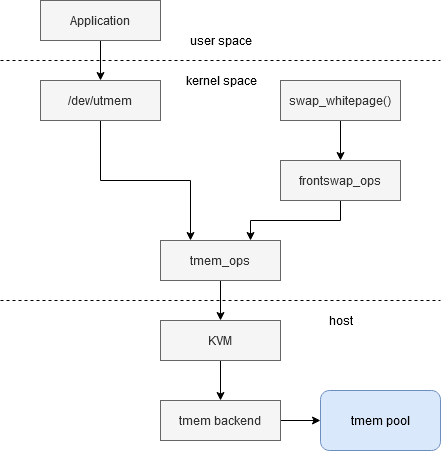
\includegraphics[width=0.7\textwidth]{pictures/utmemFlow.png}
  \caption{Δομή του \en{utmem} μηχανισμού}
  \label{fig:genUtmem}
\end{figure}

\section{Συμπεράσματα - Στόχος της εργασίας}

Πλέον είναι σαφές ότι η \en{utmem} είναι κατάλληλη λύση για περιπτώσεις
\en{virtualization} όπου υπάρχει πίεση μνήμης, ή έχει δοθεί ελάχιστη στο
\en{guest} σύστημα. Η εκτέλεση υπηρεσιών ως \en{unikernels}, είναι ένα συνηθισμένο
παράδειγμα ελάχιστης διαθέσιμης μνήμης, όπου θα ταίριαζε ένας μηχανισμός
ανταλλαγής μνήμης με τον \en{host}, όπως η \en{utmem}. Σκοπός αυτής της εργασίας
είναι να ενσωματώσουμε τον μηχανισμό \en{utmem} στο \en{Rumprun unikernel framework}.
Επίσης, όπως θα φανεί και στην συνέχεια, εκτιμάται η χρηστική αξία και οι επιδόσεις του
συνδυασμού των προαναφερθέντων τεχνολογιών.
